%****************************************************************************************************************
\section{Introducción}
\begin{frame}
	\frametitle{Contenido}
	\tableofcontents[currentsection,hideothersubsections]
\end{frame}

%================================================================================================================
\subsection{Motivación}
\begin{frame}
	\frametitle{Motivación}
	\begin{figure}
		\begin{center}
			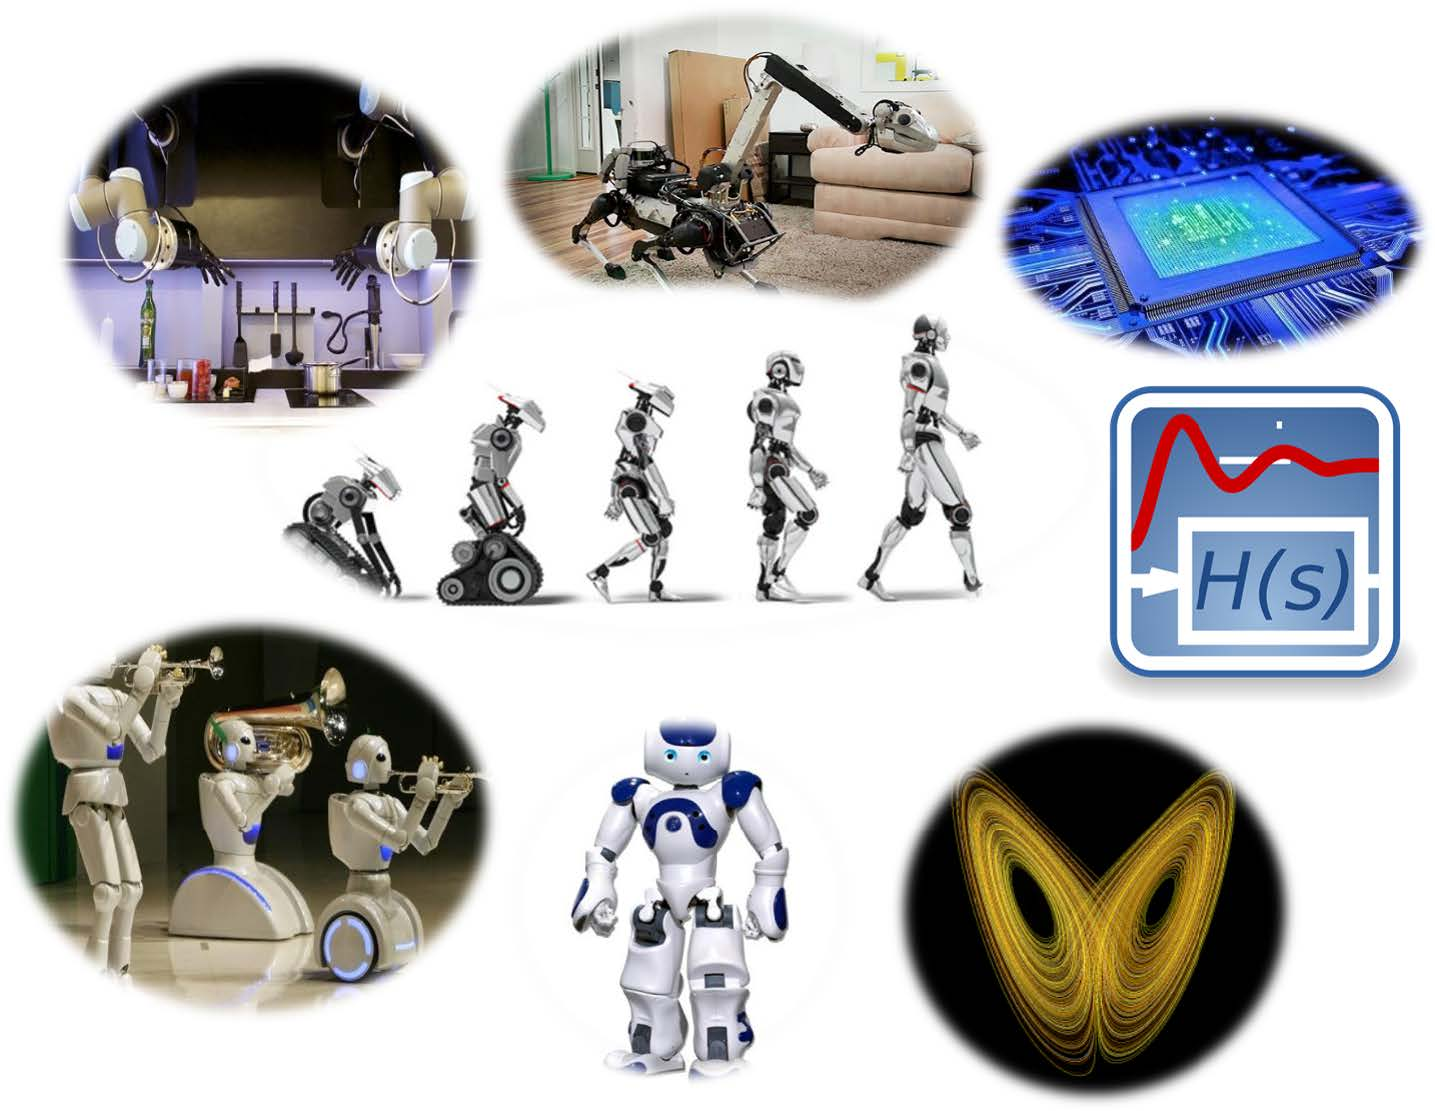
\includegraphics[scale=1]{Introduccion/motivacion.jpg}  
		\end{center}
	\end{figure}
\end{frame}

%================================================================================================================
\subsection{Robots Manipuladores}
\begin{frame}[shrink=20]{Robots Manipuladores}
	\begin{block}{}
		Presenta la capacidad para la manipulación de:
		\begin{itemize}
			\item Materiales.
			\item Piezas.
			\item Herramientas.
			\item Dispositivos.
		\end{itemize}
	\end{block}
	
	\vspace{0.4cm}
	\begin{columns}[T]
		\begin{column}{.33\textwidth}
			\begin{block}{\small{Robot manipulador industrial}}
				\centering
				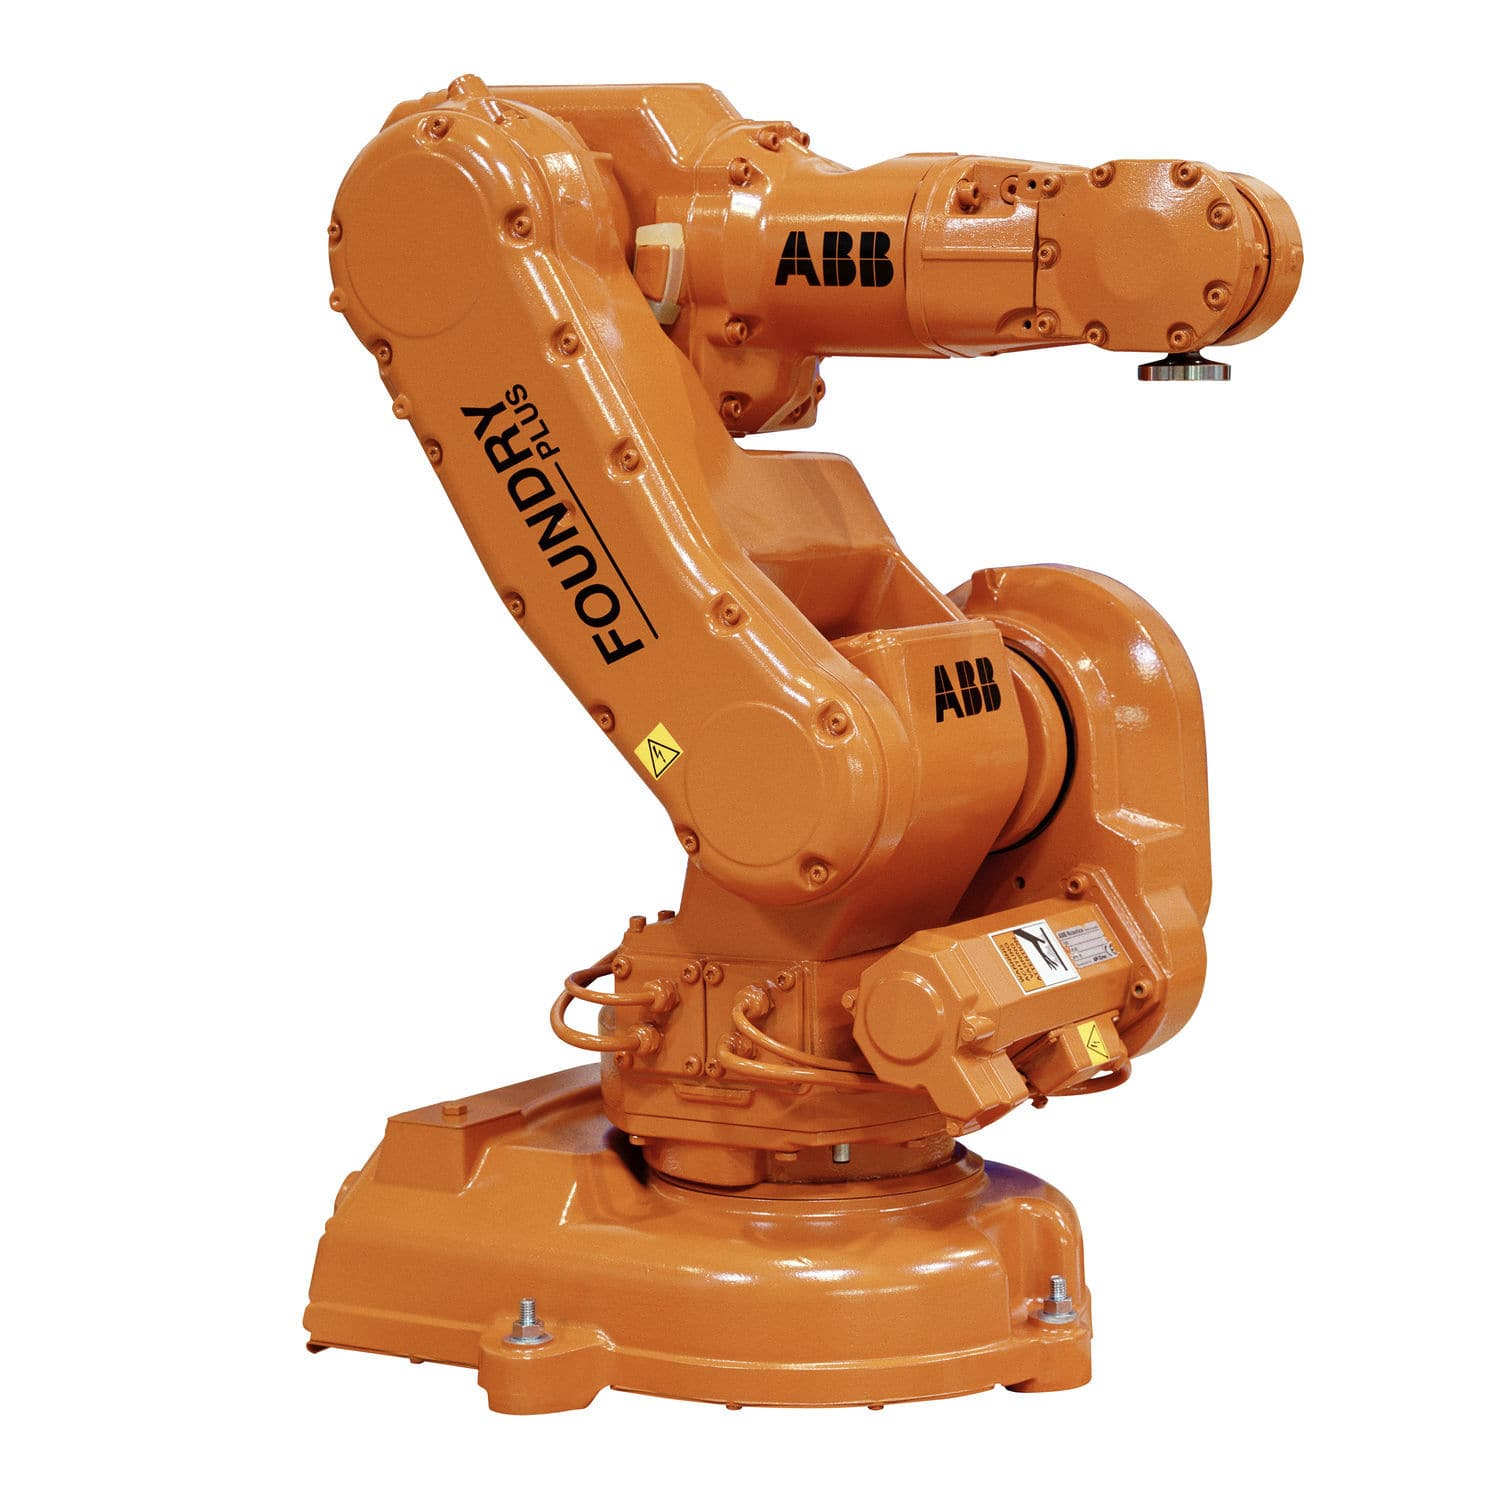
\includegraphics[height=4cm,width=4cm]{Introduccion/ind-robot.jpg}
			\end{block}
		\end{column}
		
		\begin{column}{.33\textwidth}
			\begin{block}{\small{Robot manipulador cirujano}}	
				\centering
				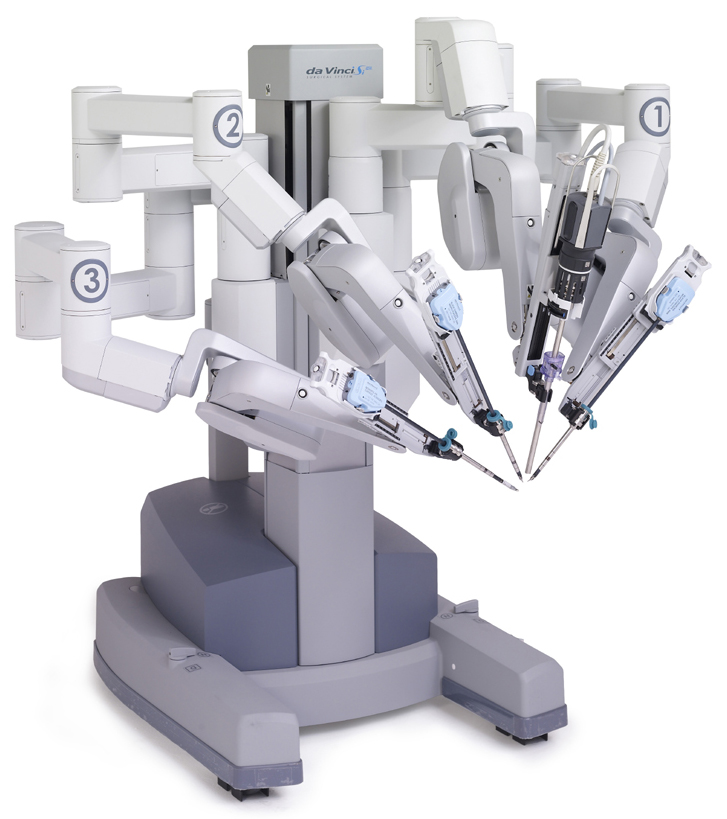
\includegraphics[height=4cm,width=4cm]{Introduccion/med-robot.jpg}
			\end{block}
		\end{column}
		\begin{column}{.33\textwidth}
			\begin{block}{\small{Robot manipulador de servicio}}
				\scriptsize
				\centering
				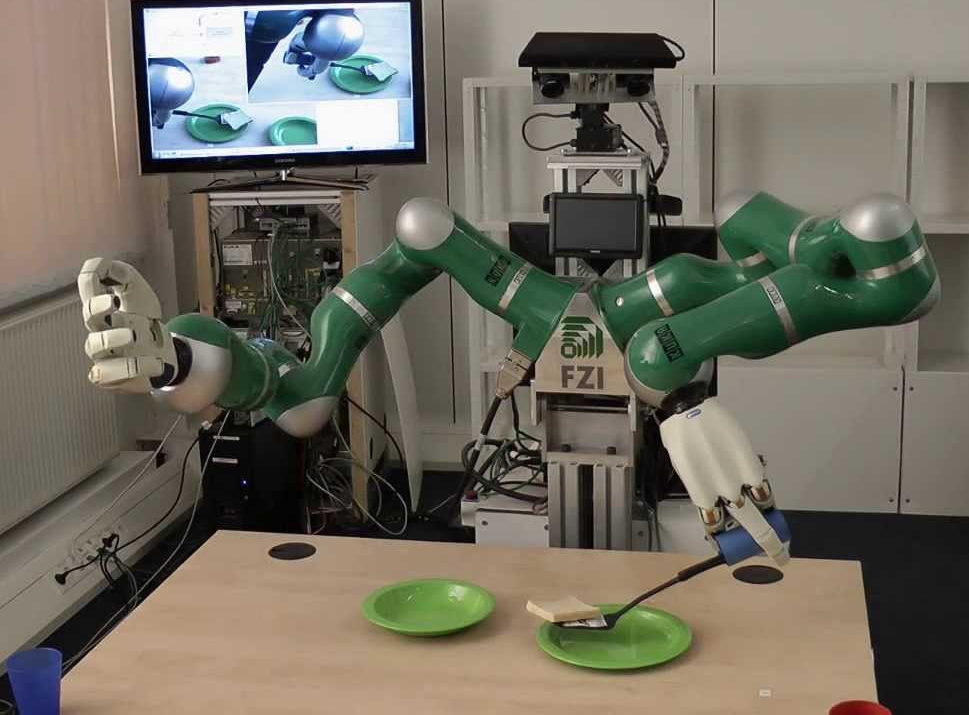
\includegraphics[height=4cm,width=4cm]{Introduccion/serv-robot.jpg}
			\end{block}
		\end{column}
	\end{columns}
\end{frame}

%================================================================================================================
\subsection{Técnicas para la Sintonización de Controladores}
%\begin{frame}[shrink=20]{Sintonización de Controladores}
\begin{frame}{Sintonización de Controladores}
	\vspace{-0.8cm}
	\begin{figure}
		\begin{center}
			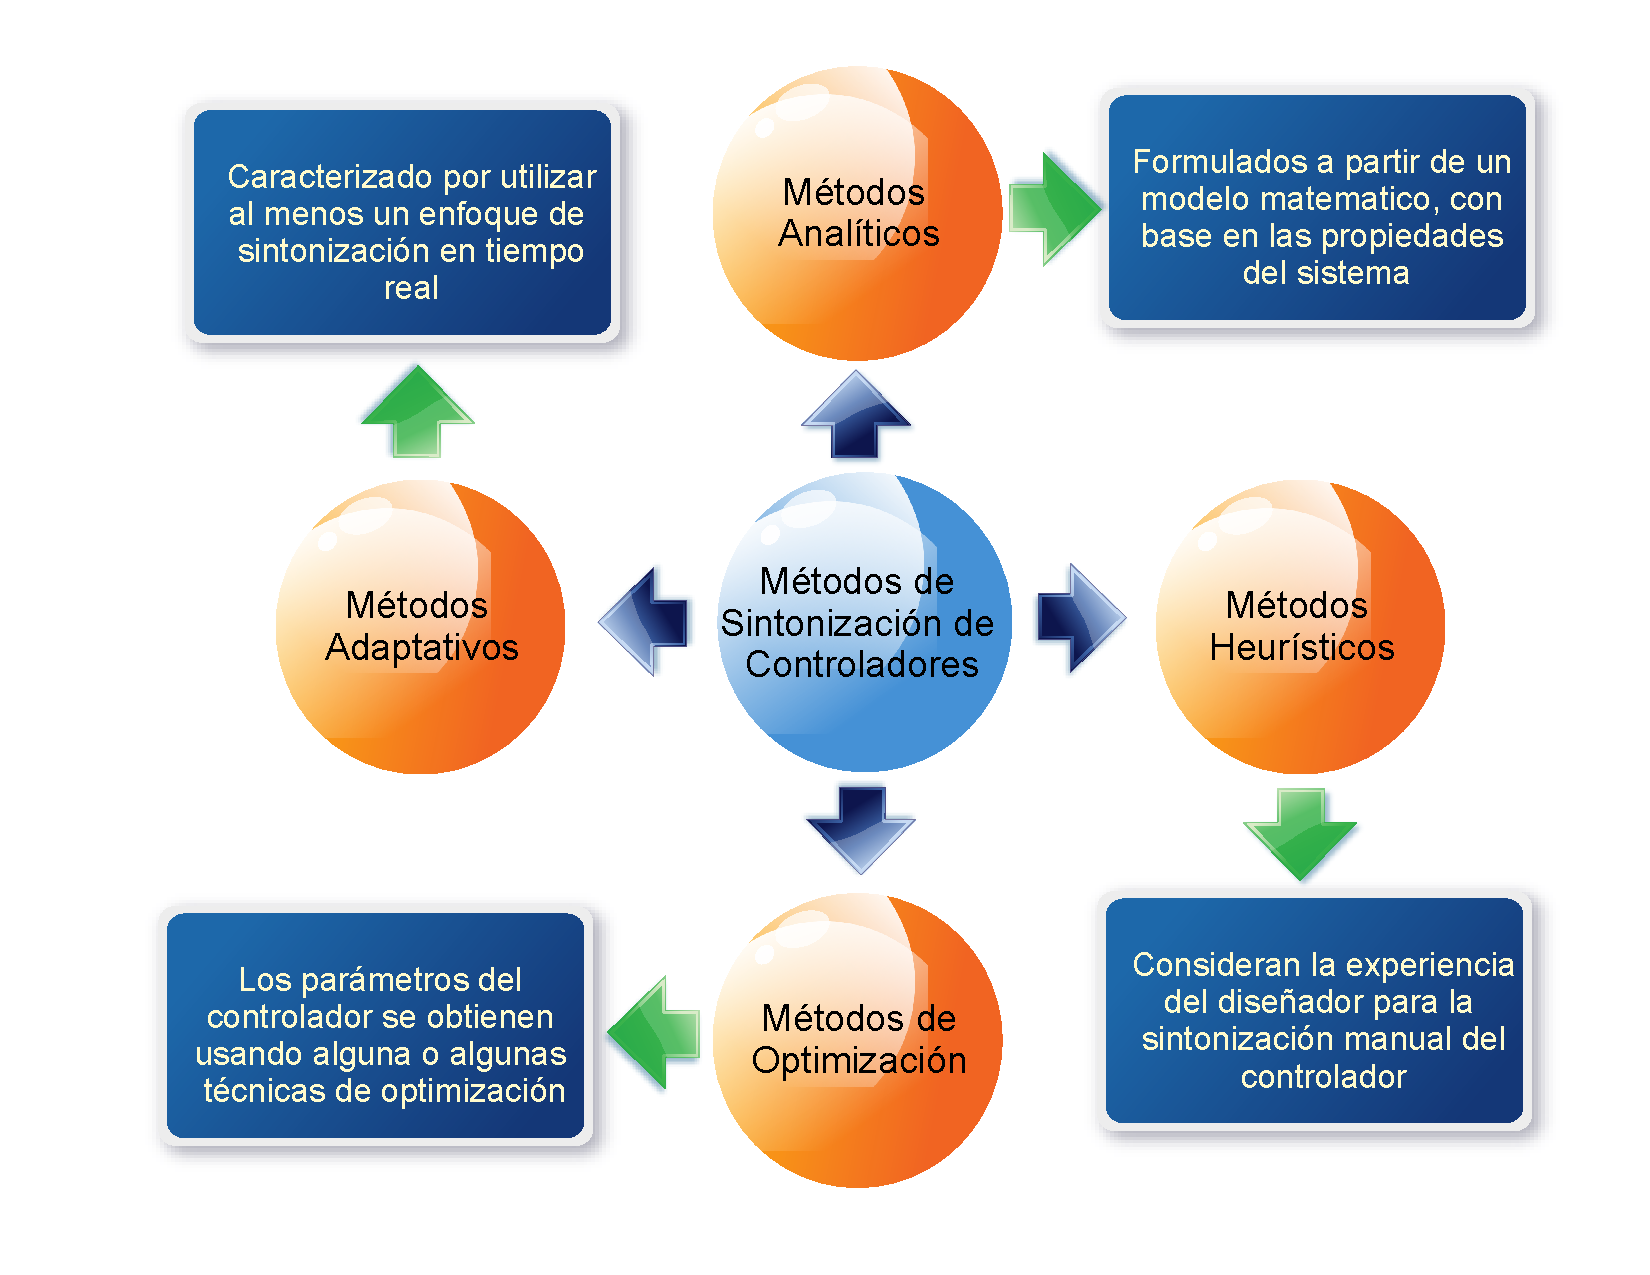
\includegraphics[scale=0.39]{Introduccion/MetSintCtrl.pdf}  
		\end{center}
	\end{figure}
\end{frame}

%***************************************************************************************************************
\subsubsection{Métodos de Optimización}
\begin{frame}[shrink=20]{Métodos de Optimización}
	\begin{block}{J. A. Romero-Perez et al, 2012}
		Se realiza una comparación entre tres métodos de auto-ajuste para un controlador PID en sistemas lineales, denominados auto-ajuste evolutivo, auto-ajuste iterativo y auto-ajuste directo.
	\end{block}
	\begin{block}{M. B. Calva Calva-Yáñez et al, 2013}
		La sintonización óptima de un controlador PI para un mecanismo de cuatro barras se presenta. Los resultados demuestran una mejora en el rendimiento del mecanismo comparado con una sintonización heurística.
	\end{block}
	\begin{block}{O. Djaneye-Boundjou et al, 2016}
		Mediante PSO se propone una metodología para la sintonización de un control PID para un robot manipulador de 2 GDL.
	\end{block}
	\begin{block}{M. G. Villarreal-Cervantes y J. Alvarez-Gallegos, 2016}
		Se presenta el ajuste de un control PID para un robot paralelo plano para el seguimiento de una trayectoria altamente no lineal. La problemática se resuelve mediante evolución diferencial.
	\end{block}
\end{frame}


%================================================================================================================
\subsection{Paradigmas del control por computadora}
\begin{frame}{Paradigmas de control por computadora}
\vspace{-0.1cm}
\centering
	\begin{block}{\small Control disparado por tiempo}
		\tiny Medición y activación del controlador cada $t_k = kT, ~ k = 1,2,3....$
	\begin{itemize}
		\tiny
		\item Emulación de control en tiempo continuo.
		\item Control en tiempo discreto.
	\end{itemize}
	\end{block}	
	\vspace{-0.2cm}
	\begin{figure}
		\begin{center}
			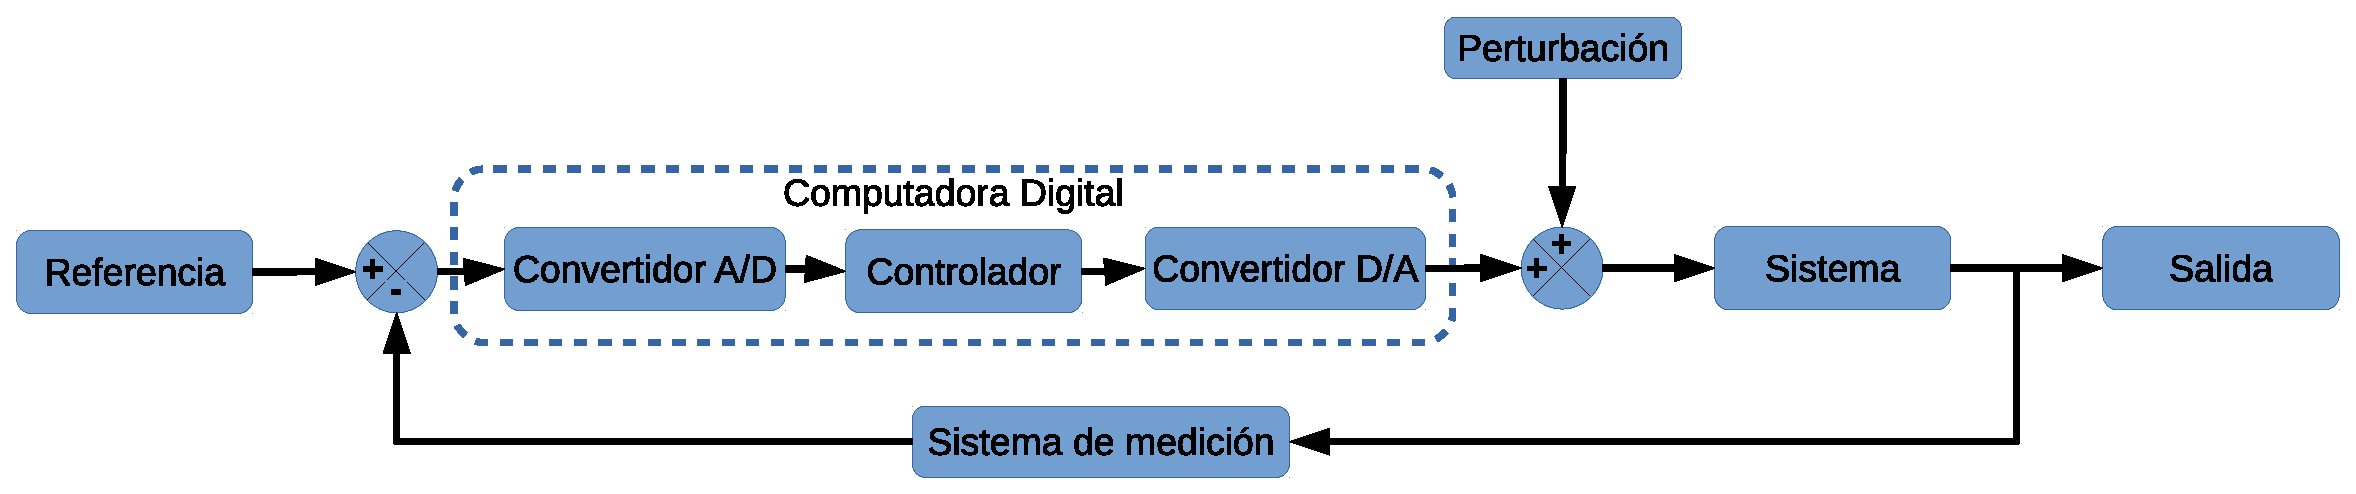
\includegraphics[scale=0.25]{Introduccion/EsqCtrlDispTiempDisc.eps}  
		\end{center}
	\end{figure}
	\begin{figure}
		\begin{center}
			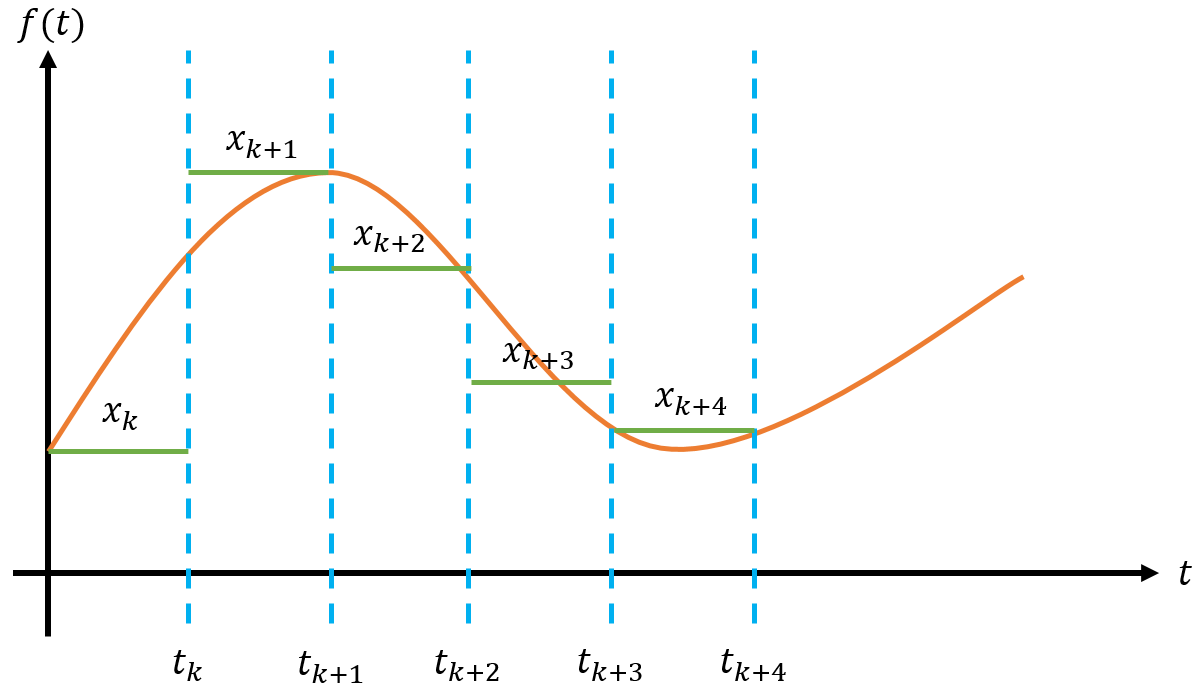
\includegraphics[scale=0.25]{Introduccion/senal-sinc.png}  
		\end{center}
	\end{figure}
\end{frame}

%================================================================================================================
\subsubsection{Paradigmas del control por computadora}
\begin{frame}[shrink=25]{Paradigmas de control por computadora}
	\vspace{-0.1cm}
	\centering
	\begin{block}{Control disparado por eventos}
		\begin{itemize}
			\item Medición de los parámetros del sistema cada $t_k = kT, ~ k = 1,2,3....$.
			\item Activación del controlador siempre que un evento suceda.
		\end{itemize}
	\end{block}	
%	\begin{figure}
%		\begin{center}
%			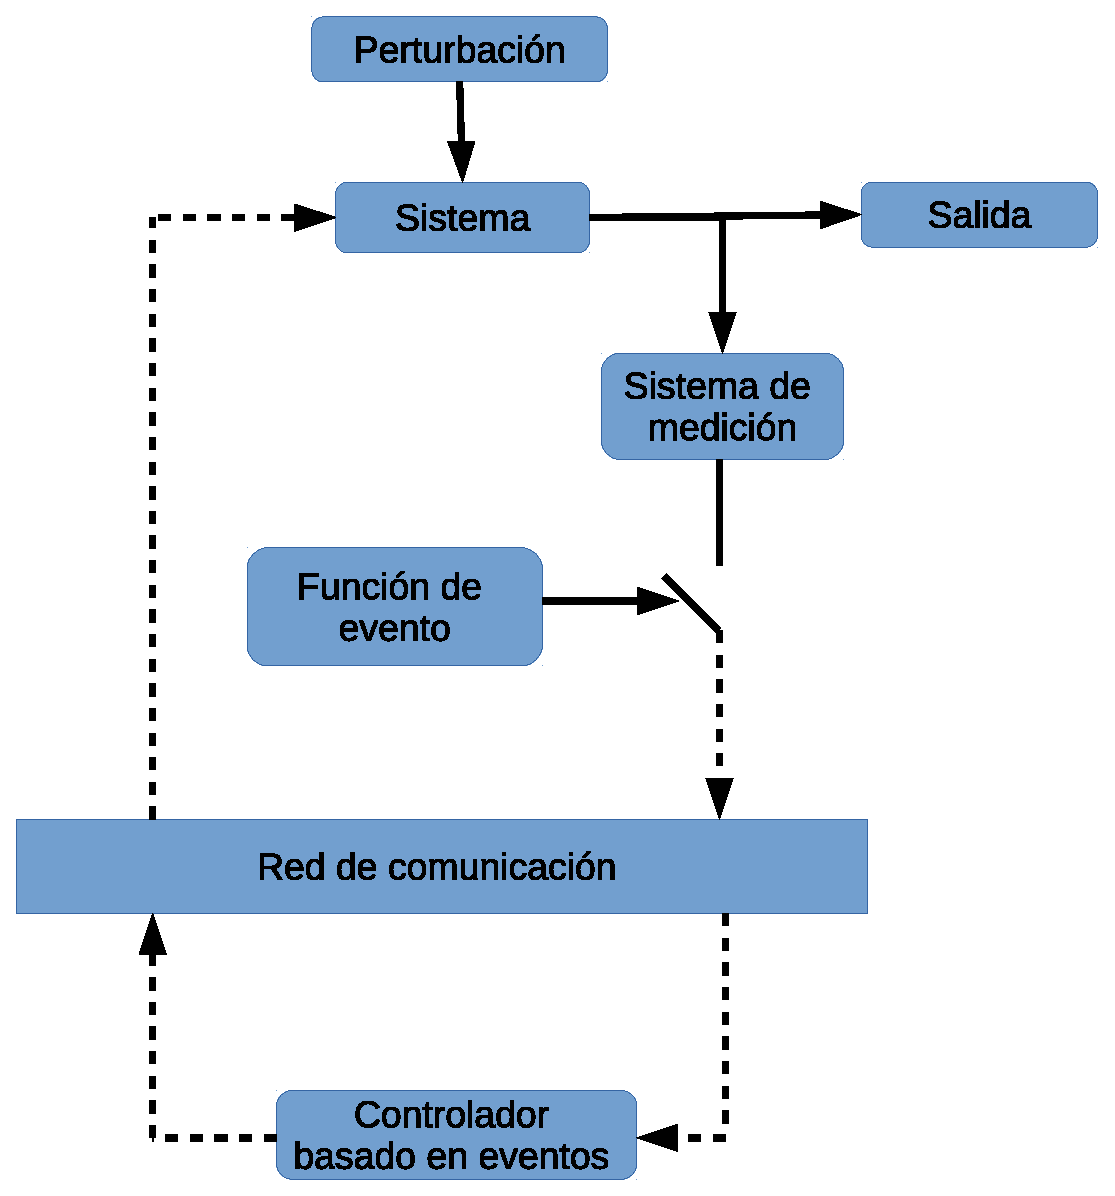
\includegraphics[scale=0.4]{Introduccion/EsqCtrlDispEvent.eps}  
%		\end{center}
%	\end{figure}

	\begin{columns}[T]
		\begin{column}{0.5\textwidth}
			\centering
			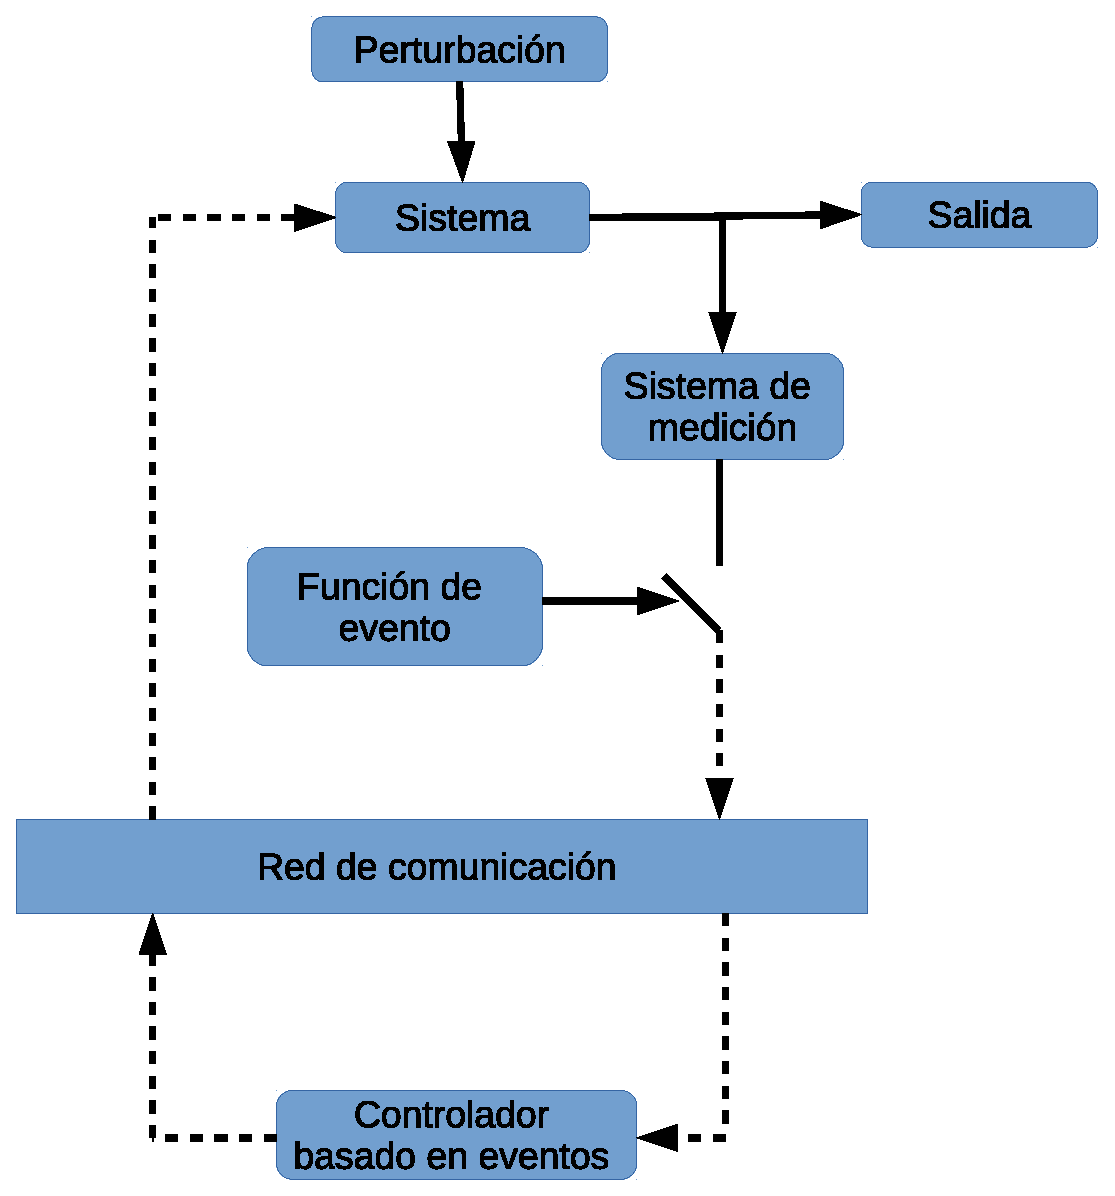
\includegraphics[scale=0.4]{Introduccion/EsqCtrlDispEvent.eps}
		\end{column}
		
		\begin{column}{0.5\textwidth}
			\vspace{2.5cm}
			\centering
			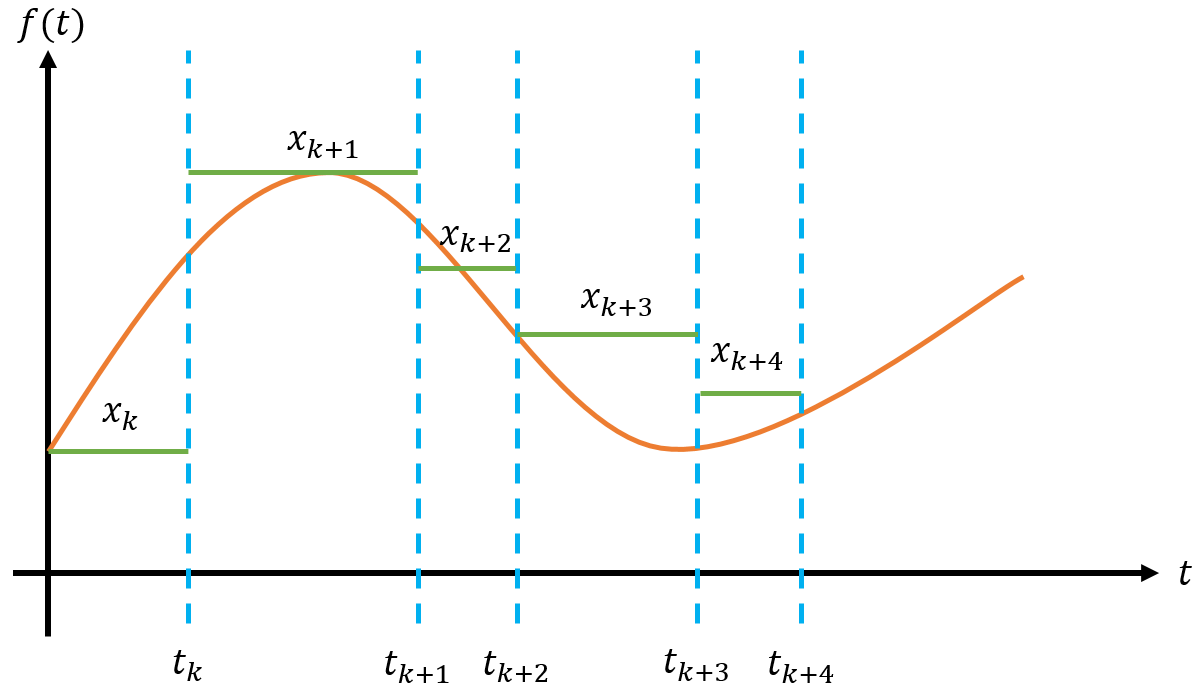
\includegraphics[scale=0.35]{Introduccion/senal-asinc.png}
		\end{column}
	\end{columns}
\end{frame}

%================================================================================================================
\subsubsection{Control disparado por eventos}
\begin{frame}[shrink=25]{Control disparado por eventos}
	\begin{block}{Miguel G.Villarreal-Cervantes et al, 2015}
		Estabilización de un robot móvil (3,0) mediante una formulación con base un análisis de estabilidad de Lyapunov. Actualización de la ley de control reducida en un $23.73\%$.
	\end{block}
	\begin{block}{Sylvain Durand et al, 2014}
		Se muestra la estabilización de un cuadricóptero en una red de comunicación. Se reduce el computo de la ley de control se reduce en un $30\%$ y $50\%$.
	\end{block}
	\begin{block}{Sylvain Durand et al, 2013}
		Se propone la estabilización de un péndulo invertido mediante una estrategia de control disparada por eventos y un mecanismo de activación basada en un enfoque de estabilidad de Lyapunov. Presenta una reducción en el número de llamadas a la estrategia de control aproximadamente del $98\%$ y $50º\%$
	\end{block}
	\begin{block}{Sylvain Durand et al, 2014}
		Se plantea un mecanismo de evento para un control robusto.	Implementado numéricamente en un robot SCARA de dos grados de libertad. Error siempre dentro del umbral propuesto para el mecanismo de eventos. Muestra una convergencia a cero cuando el tiempo tiende a infinito
	\end{block}
	
\end{frame}

%****************************************************************************************************************
\section{Planteamiento del problema}{
	\begin{frame}
		\frametitle{Contenido}
		\tableofcontents[currentsection,hideothersubsections]
	\end{frame}

%================================================================================================================
\subsection{Planteamiento del problema}
\begin{frame}[shrink=20]{Planteamiento del problema}
	\centering
\begin{block}{}
	\justifying
	Considerando el problema de regulación para un robot manipulador se plantea lo siguiente:
	\begin{itemize}
		\item La sintonización óptima de un controlador disparado por eventos.
		\item Minimiza el tiempo de convergencia del error cuando este tiende a cero.
		\item Mecanismo de evento basado en un intervalo de error deseado.
	\end{itemize}
\end{block}
	\centering
	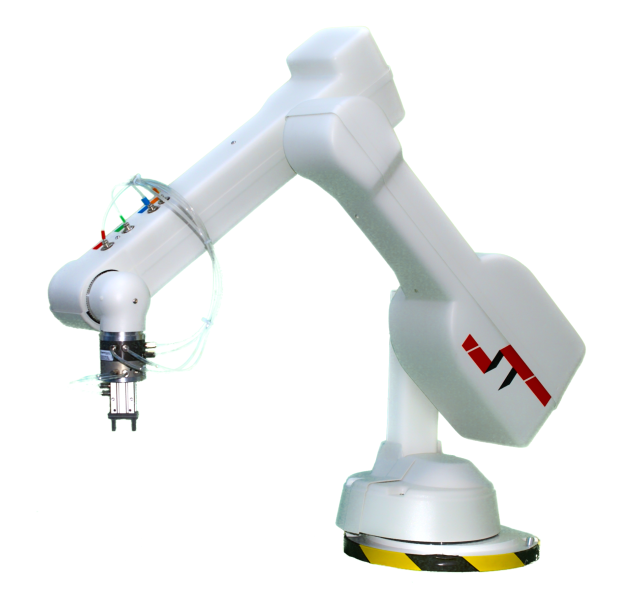
\includegraphics[scale=0.3]{Introduccion/arm-rob.png}
\end{frame}

%****************************************************************************************************************
\section{Objetivos}{
	\begin{frame}
		\frametitle{Contenido}
		\tableofcontents[currentsection,hideothersubsections]
	\end{frame}
%================================================================================================================
\subsection{Objetivos}
\begin{frame}[shrink=20]{Objetivos}
\begin{block}{Objetivo general}
	\begin{itemize}
		\justifying
		\item Actualizar de forma óptima la señal de control generada a partir del enfoque de control disparado por evento con el propósito de garantizar un desempeño apropiado en la realización de tareas desarrolladas por un robot manipulador.
	\end{itemize}
\end{block}
\begin{block}{Objetivos particulares}
	\justifying
	\begin{itemize}
		\item Desarrollar el enfoque de control basado en eventos en un robot manipulador de tres grados de libertad.
		\item Establecer el problema de optimización que resuelve el objetivo general del proyecto.
		\item Resolver el problema con alguna técnica de optimización.
	\end{itemize}
\end{block}
\end{frame}

%****************************************************************************************************************
\section{Justificación}{
	\begin{frame}
		\frametitle{Contenido}
		\tableofcontents[currentsection,hideothersubsections]
	\end{frame}
%================================================================================================================
\subsection{Justificación}
\begin{frame}[shrink=20]{Justificación}
\begin{block}{}
	\justifying
	\begin{itemize}
		\justifying
		\item La aplicación del control disparado por eventos en un robot manipulador asegura la disminución en la carga computacional y a su vez disminuye el consumo energético, lo que en consecuencia produce un menor costo.
		\item La importancia de este trabajo de investigación radica en la sintonización de los parámetros de un controlador disparado por eventos para un robot manipulador, de tal manera que el sistema presente un rendimiento aceptable bajo un tiempo y margen de error deseados.
	\end{itemize}
\end{block} 
	\vspace{0.2cm}
	\centering
	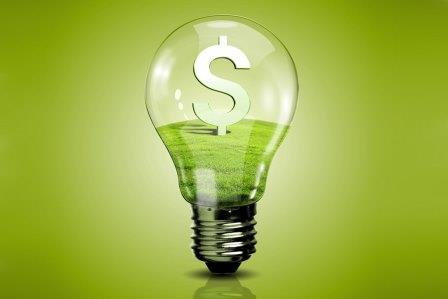
\includegraphics[scale=0.4]{Introduccion/costo-energ.jpg}
\end{frame}

%****************************************************************************************************************
\section{Metodología}{
	\begin{frame}
		\frametitle{Contenido}
		\tableofcontents[currentsection,hideothersubsections]
	\end{frame}
%================================================================================================================
\subsection{Metas} 
\begin{frame}[shrink=20]{Metas Periodo 2017/02}
%	\vskip0.5cm
	\begin{block}{Metas} 			
		\justifying	
		Con el propósito de desarrollar y lograr los objetivos del presente trabajo de investigacion se plantean las siguientes metas:	
		\begin{itemize}
			\item [I)] Obtención del modelo dinámico del robot manipulador.
			\item [II)] Planteamiento y desarrollo del controlador disparado por eventos.
			\item [III)] Puesta en marcha del prototipo experimental.
			\item [IV)] Escritura formal obtención y formulación modelo dinámico y del controlador propuesto.
			\item [V)] Formulación del problema de optimización.
		\end{itemize}
	\end{block}
	\begin{table}[H]
		\centering
		\begin{tabular}{|c|c|c|c|c|c|}
			\hline
			\multicolumn{6}{|c|}{Periodo 2017/02}\\\hline\hline
			Metas 	& Agosto 	& Septiembre 	& Octubre 	& Noviembre & Diciembre \\\hline
			I 		& X 		& X 			& X 		& X 		& 			\\\hline
			II		& X 		& X 			& X 		& X 		& 			\\\hline
			III		& 			&				&			& X			& X			\\\hline
			IV		&			&				&			&			& X			\\\hline
			V		&			&				&			&			& X			\\\hline
		\end{tabular}
		
%		\caption{Cronograma de Actividades I} \label{reglasI}
	\end{table}
\end{frame}

\subsubsection{Metodología} 
\begin{frame}[shrink=20]{Metas Periodo 2018/01}
	%	\vskip0.5cm
	\begin{block}{Metas} 			
		\justifying		
		\begin{itemize}
			\item [VI)] Resolución del problema de optimización bajo alguna técnica de optimización.
			\item [VII)] Validación del los resultados de forma numérica.
			\item [VIII)] Divulgación del trabajo de investigación en congresos o revistas nacionales o internacionales.  
			\item [IX)] Escritura de los resultados del problema de optimización y su solución.
		\end{itemize}
	\end{block}
	\begin{table}[H]
		\centering
		\begin{tabular}{|c|c|c|c|c|c|c|}
			\hline
			\multicolumn{7}{|c|}{Periodo 2018/01}\\\hline\hline
			Metas 	& Enero & Febrero 	& Marzo & Abril & Mayo	& Junio \\\hline
			V 		& X 	& X 		& X 	& 	 	&  		& 		\\\hline
			VI 		& 	 	& 			& X	 	& X 	& X 	& 		\\\hline
			VII		& 		& 			&		& X		& X		& 		\\\hline
			VIII	&		&			&		& 		& X		& X		\\\hline
			IX		&		&			&		&		&		& X		\\\hline
		\end{tabular}
%		\caption{Conograma de Actividades II} \label{reglasII}
	\end{table}
\end{frame}

\subsubsection{Metodología} 
\begin{frame}[shrink=20]{Metas Periodo 2018/02}
	%	\vskip0.5cm
	\begin{block}{Metas} 			
		\justifying		
		\begin{itemize}
			\item [X)] Validación de resultados de forma experimental.
			\item [XI)] Escritura de los resultados experimentales y terminación de documento de tesis.
			\item [XII)] Presentación del trabajo de tesis.
		\end{itemize}
	\end{block}
	
	\begin{table}[H]
		\centering
		\begin{tabular}{|c|c|c|c|c|c|}
			\hline
			\multicolumn{6}{|c|}{Periodo 2018/02}\\\hline\hline
			Metas 	& Agosto 	& Septiembre 	& Octubre 	& Noviembre & Diciembre \\\hline
			X		& X 		& X 			& 	 		&  			& 			\\\hline
			XI		& 			&				& X			& 			& 			\\\hline
			XII		&			&				& X			& X			& X			\\\hline
		\end{tabular}
		\caption{Cronograma de Actividades III} \label{reglasIII}
	\end{table}%
\end{frame}